\section{Simplified Spherical Harmonics}\label{appsec:SPn}

First, the SP$_3$ method will be derived from equation \ref{e:multigroupboltzmann}.  From these results, simplifications can be made to easily obtain the SP$_1$ equations as well.

\subsection{SP$_3$}\label{appsubsec:SP3}



\subsection{SP$_1$}\label{appsubsec:SP1}



\section{Method of Collision Probabilities}\label{appsec:CP}



\subsection{Derivation}\label{appsubsec:CPderivation}

To derive the transport matrix for a cylindrical pin cell, we begin by considering the fraction of neutrons from a point source which will reach a line whose closest distance to the point source is $\tau$ mean free paths.  We will consider the point source to be an isotropic unit point source.  The polar angle is $\theta$ and the azimuthal angle is $\alpha$.  The fraction of neutrons emitted into a specific direction $d\Omega$ about $\bm{\Omega$} from the point source to the line in question is given by,

\begin{equation}
\frac{d\Omega}{4\pi} = \frac{sin\left(\theta\right)d\theta d\alpha}{4\pi}.
\end{equation}

Integrating this expression over the polar angle gives the probability that neutrons will be emitted from the source in $d\alpha$ about $\alpha$ and reach the line a distance of $\tau$ away:

\begin{equation}
\intop_0^\pi e^{-\frac{\tau}{\sin\theta}} \frac{\sin\theta d\theta d\alpha}{4\pi}
\end{equation}

We are only concerned with the fraction of neutrons in $d\alpha$ which are also in $d\Omega$.  The fraction of neutrons emitted into $d\alpha$ is given by $\frac{d\alpha}{2\pi}$, so if we divide the previous expression by this fraction, we obtain the probability that a neutron emitted form the source in direction $d\alpha$ about $\alpha$ will reach the line:

\begin{align}\label{e:CPprobLine}
p\left(\tau\right) &= \frac{1}{2} \intop_0^\pi e^{-\frac{\tau}{\sin\theta}} \sin\theta d\theta \nonumber\\
 &= \intop_0^{\frac{\pi}{2}} e^{-\frac{\tau}{\sin\theta}}\sin\theta d\theta \nonumber\\
 &= Ki_2\left(\tau\right)
\end{align}

where $Ki_2\left(x\right)$ is the second-order Bickley-Naylor function\todo{cite}.  The Bickley-Naylor function can be defined as follows:

\begin{subequations}\label{e:BickleyFunctions}
  \begin{equation}
  Ki_n\left(x\right) = \intop_0^{\frac{\pi}{2}} \cos^{n-1}\theta e^{-\frac{x}{\cos\theta}} d\theta
  \end{equation}
  \begin{equation}
  \frac{dKi_n\left(x\right)}{dx} = -Ki_{n-1}\left(x\right)
  \end{equation}
  \begin{equation}
  \intop_a^b Ki_n\left(y\right) dy = Ki_{n+1}\left(a\right)-Ki_{n+1}\left(b\right)
  \end{equation}
\end{subequations}

Using equations \ref{e:CPprobLine} and \ref{e:BickleyFunctions}, we can now determine the probability of a neutron which escapes from region $i$ having its next collision in region $j$.  This probability is given by the probability of the escaped neutron reaching the first edge of region $j$ minus the probability of reaching the second edge of $j$:

\begin{equation}\label{e:CPpTauAlphaY}
p_{ij}\left(\tau, \alpha, y\right) = Ki_2\left(\tau_{ij} + \tau_j + \tau\right) - Ki_2\left(\tau_{ij} + \tau\right)
\end{equation}

where $\tau_{ij}$ is the number of mean free paths between $i$ and $j$, $\tau_j$ is the number of mean free paths across $j$, and $\tau$ is the number of mean free paths from the neutron's point of emission to the edge of region $i$.  The variable $y$ is defined along an axis in the plane of the problem perpendicular to the direction of streaming.  The combination of $\tau$ and $y$ specify a specific point in region $i$ for each angle $\alpha$.

Next, we define a strip in $i$ of length $t_i = \frac{\tau}{\Sigma_i}$ along the streaming direction with width $dy$.  To obtain the fraction of neutrons born in this strip that collide in $j$, we integrate the strip and divide by its length:

\begin{align}
p_{ij}\left(\alpha, y\right) &= \frac{1}{t_i} \intop_0^{t_i} p_{ij}\left(\tau, \alpha, y\right) dt \nonumber \\
&= \frac{1}{t_i} \intop_0^{t_i} Ki_2\left(\tau_{ij} + \tau\right) - Ki_2\left(\tau_{ij} + \tau_j + \tau\right) dt \nonumber \\
&= \frac{1}{t_i} \intop_0^{t_i} Ki_2\left(\tau_{ij} + \tau_i - \Sigma_i t\right) - Ki_2\left(\tau_{ij} + \tau_j + \tau_i - \Sigma_i t\right) dt
\end{align}

Now we apply a change of variables $x=\tau_{ij} + \tau_i - \Sigma_i t$.  Doing this, we obtain

\begin{align}
p_{ij}\left(\alpha, y\right) &= -\frac{1}{\Sigma_i t_i} \intop_{\tau_{ij} + \tau_i}^{\tau_{ij}} Ki_2\left(x\right) - Ki_2\left(x + \tau_j\right) dx \nonumber \\
&= \frac{1}{\Sigma_i t_i} \left[\left(Ki_3\left(\tau_{ij}\right) - Ki_3\left(\tau_{ij} + \tau_i\right)\right) - \left(Ki_3\left(\tau_{ij} + \tau_i\right) - Ki_3\left(\tau_{ij} + \tau_i + \tau_j\right)\right)\right]
\end{align}

This expression can now be multiplied by the fraction of neutrons in each strip and integrated over $y$ to obtain the total fraction of neutrons born anywhere in $i$ that stream in direction $\alpha$ and collide in $j$.

\begin{align}
p_{ij}\left(\alpha\right) &= \intop_{y_{min}\left(\alpha\right)}^{y_{max}\left(\alpha\right)} p_{ij}\left(\alpha,y\right) \frac{t_i}{V_i} dy \nonumber\\
&= \frac{1}{\Sigma_i V_i} \intop_{y_{min}\left(\alpha\right)}^{y_{max}\left(\alpha\right)} \left[\left(Ki_3\left(\tau_{ij}\right) + Ki_3\left(\tau_{ij} + \tau_i + \tau_j\right)\right) - \left(Ki_3\left(\tau_{ij} + \tau_i\right) + \left(Ki_3\left(\tau_{ij} + \tau_j\right)\right)\right)\right] dy
\end{align}

Finally, we obtain element $ij$ of the transport matrix by multiplying by the volume and cross-section.  When multiplied by $\phi_i$, this gives the total contribution to $\phi_j$ from region $i$.

\begin{align}\label{e:CPPij}
P_{ij}\left(\alpha\right) &= \Sigma_i V_i p_{ij}\left(\alpha\right) \nonumber \\
&= \intop_{y_{min}\left(\alpha\right)}^{y_{max}\left(\alpha\right)} \left[\left(Ki_3\left(\tau_{ij}\right) + Ki_3\left(\tau_{ij} + \tau_i + \tau_j\right)\right) - \left(Ki_3\left(\tau_{ij} + \tau_i\right) + \left(Ki_3\left(\tau_{ij} + \tau_j\right)\right)\right)\right] dy
\end{align}

Now that this probability has been derived, it can be integrated over all $\alpha$ to obtain the transport matrix elements for a specific geometry.

We must also handle the self-transport case, where $i=j$.  Again we follow the same procedure and define the probability $p_{ii}\left(t, \alpha, y\right)$ as the probability the neutron reaches region $i$ minus the probability it escapes region $i$.  Since the neutron was born in region $i$, the first probability is 1.  This gives the following expressions:

\begin{subequations}\label{e:CPPii}
  \begin{align}
  p_{ii}\left(t,\alpha,y\right) &= 1 - Ki_2\left(\tau\right) \\
  p_{ii}\left(\alpha,y\right) &= \frac{1}{t_i} \intop_0^{t_i} p_{ii}\left(t,\alpha,y\right) dt \nonumber \\
  &= 1- \frac{1}{\Sigma_i t_i} \left[Ki_3\left(0\right) - Ki_3\left(\tau_i\right)\right] \\
  p_{ii}\left(\alpha\right) &= \intop_{y_{min}\left(\alpha\right)}^{y_{max}\left(\alpha\right)} p_{ii}\left(\alpha,y\right) \frac{t_i dy}{V_i} \nonumber\\
  &= 1 - \frac{1}{\Sigma_i V_i} \intop_{y_{min}\left(\alpha\right)}^{y_{max}\left(\alpha\right)} \left[Ki_3\left(0\right) - Ki_3\left(\tau_i\right)\right] dy \\
  P_{ii}\left(\alpha\right) &= \Sigma_i V_i p_{ii}\left(\alpha\right) \nonumber \\
  &= \Sigma_i V_i - \intop_{y_{min}\left(\alpha\right)}^{y_{max}\left(\alpha\right)} \left[Ki_3\left(0\right) - Ki_3\left(\tau_i\right)\right] dy
  \end{align}
\end{subequations}

Now this self-transport kernel can be used with the kernel in \ref{e:CPPij} to set up the full transport matrix for a problem.  This matrix is dependent on the geometry of the problem, so it must be done for each unique problem being solved.  The following section discusses the details of this process for a cylindrical pin cell.

\subsection{CP in Cylindrical Coordinates}\label{appsubsec:CPcylCoord}

To obtain the transport matrix for a cylindrical pin cell, the pin cell must first be cylindricized.  To do this, the moderator region around the outside of the fuel pin is changed to an annular ring which preserves the total volume of the cylinder.  This allows the calculation to be 1D spatially.  Secondly, to ensure that there is a sufficient source driving the problem, a fuel and moderator mixture can be placed in a ring beyond the moderator ring.  This is especially important for using the CP method for decusping since the control rod pin cell has no fission source of its own to drive the problem.

\begin{figure}
  \centering
  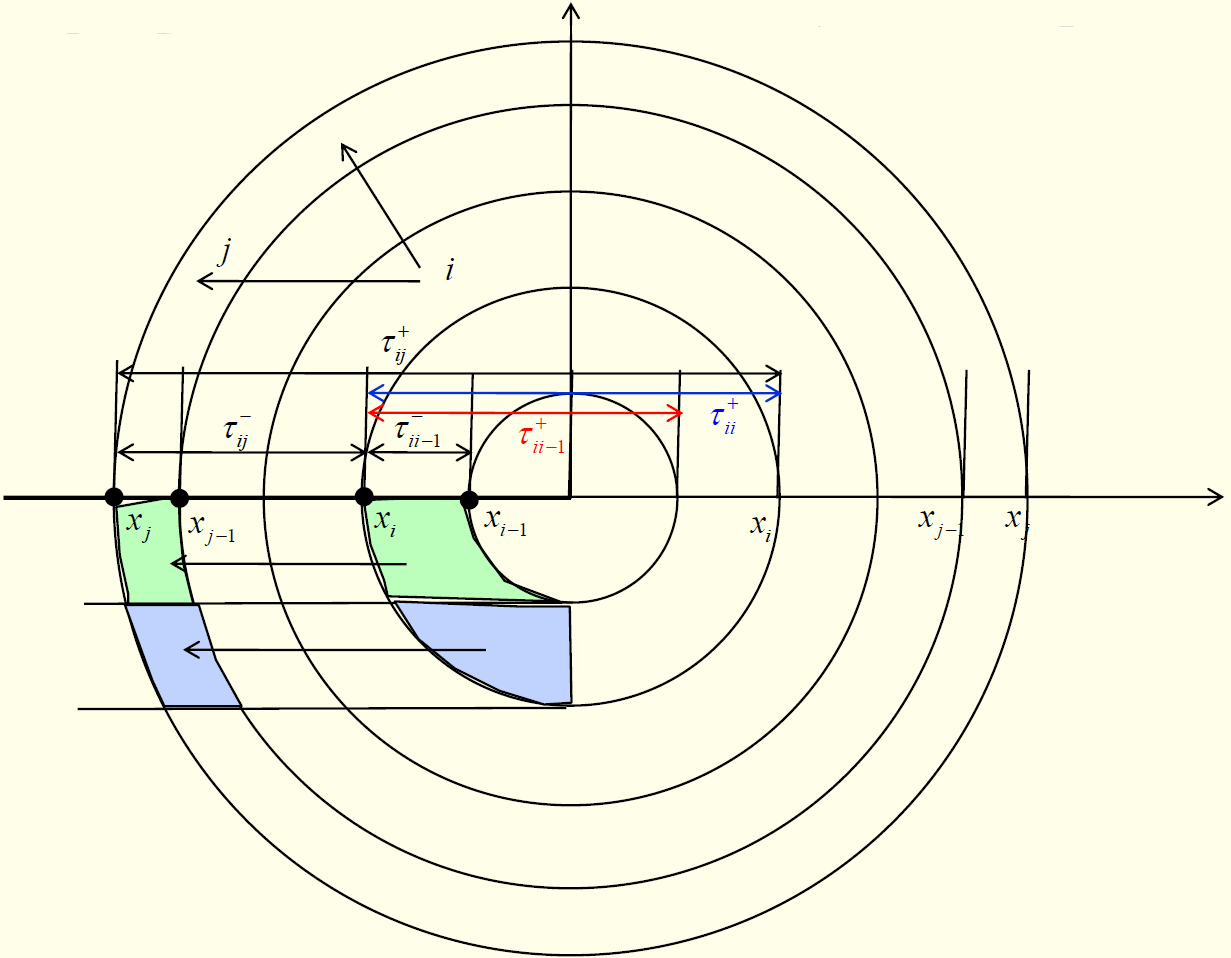
\includegraphics[width=0.8\textwidth]{figs/JooCPcylGeom.png}
  \caption{Cylindrical Geometry Collision Probabilities}\label{f:CPcylGeom}
\end{figure}
\todo{cite figure}

Now that the geometry is set up, we can take advantage of the symmetry of the problem and only model on quarter of the volume to simplify the calculation.  The kernels from equations \ref{e:CPPij} and \ref{e:CPPii} can be used, but some modification is required.  The reason for these modifications is that from a ring $i$, a ring $j$ which is outside ring $i$ can be intersected from two different directions.  Two ``sub-kernels'' are defined for teh positive and negative directions.  Each covers only one of two directions, so they should be multiplied by $\frac{1}{2}$.  However, each only accounts for $\frac{1}{4}$ the total volume, so the final expression $P_{ij}\left(y\right)$ should be multiplied by 2 to account for each of these.  The sub-kernels are each multiplied by $\frac{1}{\Sigma_i V_i}$ to account for the unit source density in the volume $V_i$ as well as a $\frac{1}{\Sigma_i}$ term that comes from the change of variables during the integration over $t_i$.  The positive and negative $\tau$ terms are shown in the geometry in \ref{f:CPcylGeom}.

\begin{subequations}\label{e:CPcylPij(y)}
  \begin{align}
  P_{ij}^-\left(y\right) &= \frac{1}{\Sigma_i V_i} \left(Ki_3\left(\tau_{ij-1}^-\right) + Ki_3\left(\tau_{i-1j}^-\right) - Ki_3\left(\tau_{ij}^-\right) - Ki_3\left(\tau_{i-1j-1}^-\right)\right) \\
  P_{ij}^+\left(y\right) &= \frac{1}{\Sigma_i V_i} \left(Ki_3\left(\tau_{i-1j-1}^+\right) + Ki_3\left(\tau_{ij}^+\right) - Ki_3\left(\tau_{i-1j}^+\right) - Ki_3\left(\tau_{ij-1}^+\right)\right) \\
  P_{ij}\left(y\right) &= 2\left(P_{ij}^-\left(y\right) + P_{ij}^+\left(y\right)\right)
  \end{align}
\end{subequations}

Now we introduce notation to simplify this expression:

\begin{subequations}\label{e:CPcypPij}
  \begin{align}
  S_{ij} &= \intop_0^{R_i} \left(Ki_3\left(\tau_{ij}^+\right) - Ki_3\left(\tau_{ij}^-\right)\right)dy \\
  \Rightarrow P_{ij} &= \Sigma_i V_i \intop_0^{R_i} P_{ij}\left(y\right)dy \nonumber \\
  &= 2\left(S_{ij} + S_{i-1j-1} - S_{ij-1} - S_{i-1j}\right)
  \end{align}
\end{subequations}

\begin{figure}
  \centering
  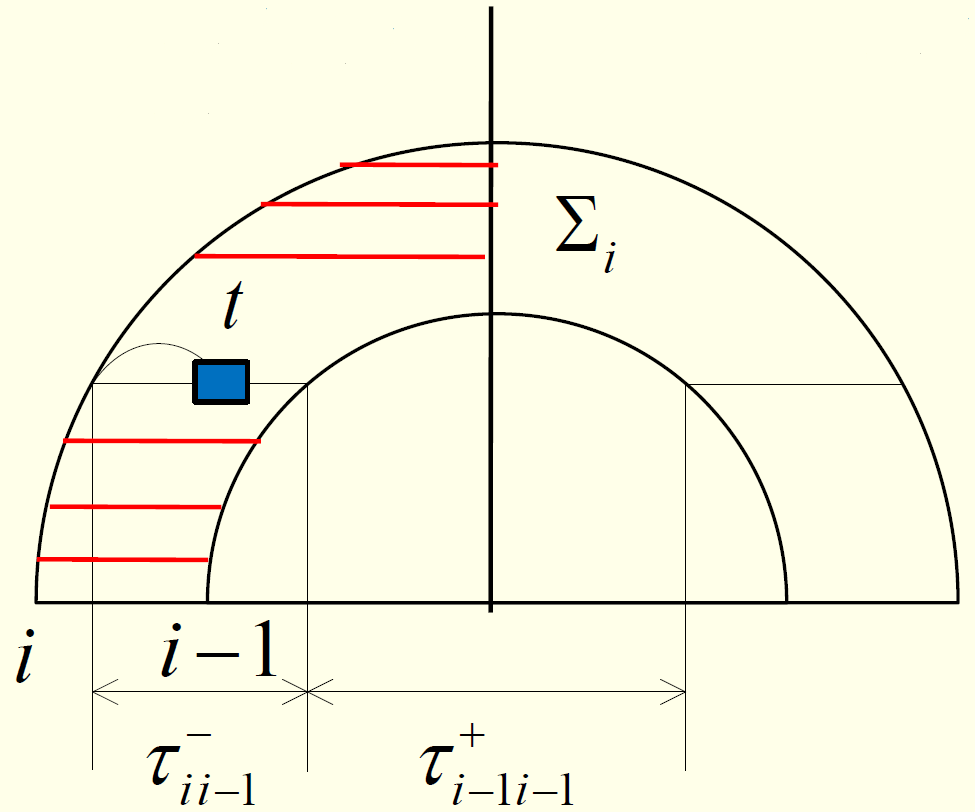
\includegraphics[width=0.6\textwidth]{figs/JooCPcylGeomSelf.png}
  \caption{Cylindrical Geometry Collision Probabilities Self-Transport}\label{f:CPcylGeomSelf}
\end{figure}

A similar process is followed for the self-transport kernel.  Again, positive and negative directions are set up.  Additionally, the possibility of a neutron being born in $i$, escaping, then re-entering the other side of $i$ must be accounted for as well.  This is illustrated in figure \ref{f:CPcylGeomSelf}.  This leads to the kernel in equation \ref{e:CPcylPii}.

\begin{subequations}\label{e:CPcylPii}
  \begin{align}
  P_{ii}^-\left(y\right) &= \frac{t_i\left(y\right)}{V_i} + \frac{1}{\Sigma_i V_i}\left(Ki_3\left(\tau_{ii-1}^-\right) + Ki_3\left(\tau_{i-1i}^-\right) - Ki_3\left(\tau_{ii}^-\right) - Ki_3\left(\tau_{i-1i-1}^-\right)\right) \\
  P_{ii}^+\left(y\right) &= \frac{t_i\left(y\right)}{V_i} + \frac{1}{\Sigma_i V_i}\left(Ki_3\left(\tau_{ii}^+\right) + Ki_3\left(\tau_{i-1i-1}^+\right) - Ki_3\left(\tau_{ii-1}^+\right) - Ki_3\left(\tau_{i-1i}^+\right)\right) \\
  P_{ii}\left(y\right) &= 2 \left(P_{ii}^-\left(y\right) + P_{ii}^+\left(y\right)\right) \\
  P_{ii} &= \Sigma_i V_i \intop_0^{R_i} P_{ii}\left(y\right) dy \nonumber \\
  &= \Sigma_i V_i  + 2\left(S{ii} + S_{i-1i-1} - S_{ii-1} - S_{i-1i}\right)
  \end{align}
\end{subequations}

$P_{ij}$ is the probability that a neutron born in cell $i$ has its first collision in cell $j$.  Likewise, $P_{ii}$ is the probability that a neutron born in cell $i$ has its first collision in the same cell.  To obtain the transport matrix elements $T_{ij}$ and $T_{ii}$, we must consider the actual linear system we wish to solve.  The goal is to find the reaction rates in each cell, from which we can easily find the flux in the cell $\phi_i$.  There are two main contributions to the reaction rates in cell $i$.  The first contribution is from neutrons born in another cell $j$ which have their first collision in cell $i$.  This source is given by $\frac{Q_j}{\Sigma_{t,j}}$, which gives the contribution to the reaction rates in $i$ when multiplied by $P_{ji}$.  The second part of the source comes from neutrons which streamed into $j$ and collided, scattered, then streamed into $i$ before having their next collision.  This source is given by $P_{ji} \phi_j c_j$, where $c_j$ is the scattering ration in cell $j$, defined as $\frac{\Sigma_{s,j}}{\Sigma_{t,j}}$.  The linear sysmem which needs to be solved is then shown in equation \ref{e:CPproblem}.

\begin{equation}\label{e:CPproblem}
\Sigma_{t,i} \phi_i V_i = sum_{j=1}^{N_R} P_{ji}\left(c_j\phi_j + \frac{Q_j}{\Sigma_{t,j}}\right)
\end{equation}

The linear system, with the matrix and source elements, can now be explicitly defined in equation \ref{e:CPlinsys}.

\begin{subequations}\label{e:CPlinsys}
  \begin{equation}
  \underline{\underline{\bm T}}\underline{\bm\phi} = \underline{\bm B}
  \end{equation}
  \begin{align}
  T_{ij} &= -P_{ji} c_j = -2 c_j \left(S_{ii} + S_{i-1j-1} - S_{ij-1} - S_{i-1j}\right) \\
  T_{ii} &= \Sigma_{t,i} V_i - P_{ii} c_i = \Sigma_{t,i} V_i - \Sigma_{s,i} V_i - 2 c_j \left(S_{ii} + S_{i-1j-1} - S_{ij-1} - S_{i-1j}\right)
  \end{align}
  \begin{equation}
  B_i =\sum_{j=1}^{N_R} P_{ji} \frac{Q_j}{\Sigma_{t,j}}
  \end{equation}
\end{subequations}

The only remaining unknowns required to construct this linear system are the $S_{ij}$ terms that involve integrals over the third-order Bickley-Naylor functions.  This will be discussed in the next section.

\subsection{Bickely-Naylor Function Integration}

In the previous sections, we defined the following functions which contain integrals over third-order Bickley-Naylor functions:

\begin{equation}\label{e:CPSijDef}
S_{ij} = \intop_0^{R} \left(Ki_3\left(\tau_{ij}^+\left(y\right)\right) - Ki_3\left(\tau_{ij}^-\left(y\right)\right)\right) dy
\end{equation}

To numerically integrate these functions, we first break them up into regions (equation \ref{e:CPSijSubInt}).

\begin{subequations}\label{e:CPSijSubInt}
  \begin{align}
  S_{ij} &= \sum_{k=1}^i S_{ij}^k \\
  S_{ij}^k &= \intop_{R_{k-1}}^{R_k} \left(Ki_3\left(\tau_{ij}^+\left(y\right)\right) - Ki_3\left(\tau_{ij}^-\left(y\right)\right)\right) dy
  \end{align}
\end{subequations}

Next, we perform a coordinate transformation to change the bounds of integration to be on the interval $\left[-1, 1\right]$.  This allows us to apply a Gaussian quadrature to evaluate the integral numerically.  The results of the transformation are shown in \ref{e:CPSijCoordTrans}, where $f\left(p\right)$ is the transformed $S_{ij}^k$ and $p_i$ and $\omega_i$ are some points and weights associated with the quadrature.

\begin{subequations}\label{e:CPSijCoordTrans}
  \begin{align}
  p &= 2\frac{y - R_{k-1}}{R_k - R_{k-1}} - 1 = 1\frac{y - R_{k-1}}{\Delta_k} -1 \\
  dp &= \frac{2}{\Delta_k}dy \\
  \Rightarrow S_{ij}^k &= \frac{\Delta_k}{2} \intop_{-1}^1 f\left(p\right)dp = \frac{\Delta_k}{2} \sum_i \omega_i f\left(p_i\right)
  \end{align}
\end{subequations}

This can now be integrated using a standard Gaussian quadrature\todo{cite}.  MPACT uses a 4-point Gaussian quadrature, shown in table \ref{t:gaussQuad}.

\begin{table}
  \centering
  \caption{Four-Point Gaussian Quadrature}\label{t:gaussQuad}
  \begin{tabular}{|c|c|}\hline
    Point & Weight \\\hline
    $\pm \sqrt{\frac{3}{7} - \frac{2}{7}\sqrt{\frac{6}{5}}}$ & $\frac{18 + \sqrt{30}}{36}$ \\\hline
    $\pm \sqrt{\frac{3}{7} + \frac{2}{7}\sqrt{\frac{6}{5}}}$ & $\frac{18 - \sqrt{30}}{36}$ \\\hline
  \end{tabular}
\end{table}

\subsection{Reciprocity}